\documentclass{report}
\usepackage[utf8]{inputenc}
\usepackage{array}
\usepackage{blindtext}
\usepackage{hyperref}
\usepackage{wrapfig}
\usepackage{multirow}
\usepackage{graphicx}
\usepackage{tabularx}
\usepackage{geometry}
\usepackage{changepage}
\usepackage{longtable}


\makeatletter
%same as \subsubsection but @level 4
\renewcommand\paragraph{\@startsection{paragraph}{4}{\z@}%
{-3.25ex\@plus -lex \@minus -.2ex}%
{1.5ex \@plus .2ex}%
{\normalfont\normalsize\bfseries}}

% number \paragraph
\setcounter{secnumdepth}{4}

\makeatother


\title{\normalsize {SOEN 6481 Summer 2021}\\[1.0cm]
\huge \textbf{\uppercase{SRS}} \\
\huge \textbf{\uppercase{e-concordia drive}}\\
\normalsize \vspace*{2\baselineskip}
}
\author{{Tavtej Singh Lehri\\
StudentID - 40121745}}
\date{August 17,2021}
%Title and Front page

\hypersetup{
    colorlinks=true,
    linkcolor=black,
    filecolor=magenta,      
    urlcolor=cyan,
    pdftitle={Delivery3 40121745},
    pdfpagemode=FullScreen,
    }
    
\urlstyle{same}

\begin{document}

\maketitle

\tableofcontents
\clearpage

\chapter{Use Case Model}
\section{Introduction}
\textbf{\large Purpose}\\
The purpose of this document is the Use-Case Model comprehensively.It describes the structure of UCM and list down the actors involved and their goals in the model.\\[1cm]
\textbf{\large Scope}\\
This Use-Case Model applies to E-Concordia Drive website to be developed by the Chronos Tech Solutions. This website will help the students learn about driving to obtain their driver's permit, while staying at their home.

\section{Actor-Goal List}
\begin{longtable}{|p{3.5cm}|p{9.5cm}|}\hline
     \textbf{Actor}&\textbf{Goal}  \\ \hline
     Student&\begin{itemize}
         \item Login
         \item View Lessons
         \item Take and Submit Quizzes
     \end{itemize} \\ \hline
     Trainer&\begin{itemize}
         \item Login
         \item Submit/Update the Lesson Content
         \item Submit/Update the quizzes
     \end{itemize} \\ \hline
     Admin&\begin{itemize}
         \item Login
         \item Approve the content posted by trainer
         \item Send comments to trainers with required changes
         \item Add/Remove a user which includes students and trainers.
         \item Manage content.
     \end{itemize} \\ \hline
     \caption{Actor Goal List.\label{long}}\\
\end{longtable}


\section{Use Case Model}
\subsection{\textbf{Use Case ID:} UC001}
\textbf{Use Case:} Student Registration\\[0.3cm]
\textbf{Description:}\\
Students should be able to create an account online by filling out the personal details. After registration students will be provided 3 unique identifiers used to login\\[0.3cm]
\textbf{Level:} User Goal\\[0.3cm]
\textbf{Primary Actor:}\\
Students\\[0.3cm]
\textbf{Supporting Actor:}\\
Mobile Devices\\[0.3cm]
\textbf{Stakeholders and Interests:}\\
Students\\[0.3cm]
\textbf{Pre-Conditions:}\\
Students should have access to any mobile device and internet connection\\[0.3cm]
\textbf{Post-Conditions:}\\
Will be determined later\\[0.3cm]
\textbf{\large {Main Success Scenario:}}
\begin{enumerate}
    \item User visits the website and clicks on the sign-up button
    \item User fills in the personal details: First Name, Last Name, Date of Birth and Address
    \item User selects the license type from the drop-down list
    \item User selects the payment type as credit card/debit card and clicks submit.
    \item After the successful payment student is provided with unique File Number, Traffic Number and Student Number the combination of which will be used to login into the account.
    \item All the 3 unique numbers will be stored in EDC database along with student information for account authentication
\end{enumerate}
\textbf{Extensions:}\\
If the payment by card fails, users should be given option to either make payment by cheque, cash or Interac\\[0.3cm]
\textbf{Special Requirements:}\\
The payments using Credit/Debit needs to be secured and the system should be secure enough to prevent data leakage.\\

%UseCase 2%
\subsection{\textbf{Use Case ID:} UC002}
\textbf{Use Case:} Trainer Registration\\[0.3cm]
\textbf{Description:}\\
Trainers should be able to create an account online by filling out the personal details.\\[0.3cm]
\textbf{Level:} User Goal\\[0.3cm]
\textbf{Primary Actor:}\\
Trainer\\[0.3cm]
\textbf{Supporting Actor:}\\
Mobile Devices\\[0.3cm]
\textbf{Stakeholders and Interests:}\\
Trainers\\[0.3cm]
\textbf{Pre-Conditions:}\\
Students should have access to any mobile device and internet connection\\[0.3cm]
\textbf{Post-Conditions:}\\
Will be determined later\\[0.3cm]
\textbf{\large {Main Success Scenario:}}
\begin{enumerate}
    \item User visits the website and clicks on the sign-up button
    \item User fills in the personal details: First Name, Last Name, Date of Birth, Teacher ID, E-mail ID and Address.
    \item User chooses the username and password of their choosing.
    \item User clicks on submit and the profile goes to admin for approval.
    \item After the admin approves/rejects an email notification is sent to the trainer.
    \item The username and password(hotkey format) will be stored in EDC database for account authentication
\end{enumerate}
\textbf{\large Extensions:}
\begin{enumerate}
    \item If the username already exist then trainer has to choose a new username.
    \item Password should be of format: 1 uppercase, 1 lowercase, 1 special character and 1 numeric character.
\end{enumerate}
\textbf{\large Special Requirements:}\\
None\\

\subsection{\textbf{Use Case ID:} UC003}
\textbf{Use Case:} Read content on student dashboard\\[0.3cm]
\textbf{Description:}\\
After the student is logged in this use case will occur. It deals with what is displayed on the dashboard page\\[0.3cm]
\textbf{Level:} User Goal\\[0.3cm]
\textbf{Primary Actor:}\\
Students\\[0.3cm]
\textbf{Supporting Actor:}\\
Mobile Devices and EDC Database\\[0.3cm]
\textbf{Stakeholders and Interests:}\\
Stakeholders will be Students
Stakeholder interest will be to let students see their details on dashboard along with lesson icons\\[0.3cm]
\textbf{Pre-Conditions:}\\
Students should have registered.\\[0.3cm]
\textbf{Post-Conditions:}\\
None\\[0.3cm]
\textbf{\large {Main Success Scenario:}}
\begin{enumerate}
    \item User visits the website and Login using the 3 unique numbers provided at time of registration
    \item Website displays license type, student number, traffic number , student name, lesson icons from the trainer backend, student progress, lesson names, enrollment and expiry date etc.
    \item Students can click on the lesson icons to start it.
    \item Students can click on start again button once to lesson is complete
\end{enumerate}
\textbf{Extensions:}\\
None\\[0.3cm]
\textbf{Special Requirements:}\\
None\\

\subsection{\textbf{Use Case ID:} UC004}
\textbf{Use Case:} View videos by students\\[0.3cm]
\textbf{Description:}\\
This use case deals with students viewing the videos posted by the trainers.\\[0.3cm]
\textbf{Level:} User Goal\\[0.3cm]
\textbf{Primary Actor:}\\
Students\\[0.3cm]
\textbf{Supporting Actor:}\\
Mobile Devices and EDC Database\\[0.3cm]
\textbf{Stakeholders and Interests:}\\
Students will be stakeholders and if the videos are not available they might not be able to learn something.\\[0.3cm]
\textbf{Pre-Conditions:}\\
Students should have registered.\\[0.3cm]
\textbf{Post-Conditions:}\\
None\\[0.3cm]
\textbf{\large {Main Success Scenario:}}
\begin{enumerate}
    \item User visits the website and Login using the 3 unique numbers provided at time of registration
    \item Website dashboard page displays the video icons taken from the trainer back-end.
    \item Students clicks on the lesson icons and the website navigates them to the lesson page.
    \item lesson name will be picked from EDC database and lesson description will have any additional information necessary related to the lesson.
    \item Student clicks on the START NOW button to start the lesson.
\end{enumerate}
\textbf{Extensions:}\\
Video does not start.
\begin{enumerate}
    \item An error/broken feed message is displayed if it is because of time out.
    \item Student should check their internet connection.
    \item If there is no issue with internet contact someone at school to look at the system.
\end{enumerate}
User is logged out of the system.
\begin{enumerate}
    \item Student is logged out after being idle for 30 minutes.
    \item Repeat from step 1 of main scenario.
    \item Video will start from where student left it at.
\end{enumerate}
\textbf{Special Requirements:}
\begin{enumerate}
    \item System should be able to handle 350000 users at same time.
    \item The video screen should be interactive which means the orientation should change if the device orientation is changes.
\end{enumerate}

\subsection{\textbf{Use Case ID:} UC005}
\textbf{Use Case:} Students take quizzes\\[0.3cm]
\textbf{Description:}\\
This use case deals with students attempting the quiz posted by the trainers.\\[0.3cm]
\textbf{Level:} User Goal\\[0.3cm]
\textbf{Primary Actor:}\\
Students\\[0.3cm]
\textbf{Supporting Actor:}\\
Mobile Devices and EDC Database\\[0.3cm]
\textbf{Stakeholders and Interests:}\\
Owner and Trainer. They want quiz so that students can practice what they have learned\\[0.3cm]
\textbf{Pre-Conditions:}\\
Students should have registered.\\[0.3cm]
\textbf{Post-Conditions:}\\
\underline{Success end condition}\\
All the questions are answered.\\[0.3cm]
\underline{Failure end condition}\\
None.\\[0.3cm]
\textbf{\large {Main Success Scenario:}}
\begin{enumerate}
    \item User visits the website and Login using the 3 unique numbers provided at time of registration
    \item Website dashboard page displays the video icons taken from the trainer back-end.
    \item Students clicks on the lesson icons and the website navigates them to the lesson page.
    \item Student should complete all the slides before moving to the quiz section.
    \item Students should select the correct answers to the questions.
    \item Click FINISH after successfully answering all the questions to complete the lesson
\end{enumerate}
\textbf{Extensions:}\\
User is logged out of the system.
\begin{enumerate}
    \item Student is logged out after being idle for 30 minutes.
    \item Repeat from step 1 of main scenario.
    \item Video will start from where student left it at.
\end{enumerate}
\textbf{Special Requirements:}
\begin{enumerate}
    \item System should be able to handle 350000 users at same time.
    \item The video screen should be interactive which means the orientation should change if the device orientation is changes.
    \item Interactive screen also means that user can select the answers in a touchscreen device as well.
    \item Quiz answers should be of type true/false, select correct option, drag and match, rearrange in correct order.
\end{enumerate}

\subsection{\textbf{Use Case ID:} UC006}
\textbf{Use Case:} Create a lesson\\[0.3cm]
\textbf{Description:}\\
This use case deals with trainers creating a lesson for students.\\[0.3cm]
\textbf{Level:} User Goal\\[0.3cm]
\textbf{Primary Actor:}\\
Trainer and Admin\\[0.3cm]
\textbf{Supporting Actor:}\\
Mobile Devices and EDC Database\\[0.3cm]
\textbf{Stakeholders and Interests:}\\
Trainer and Driving school owner. School owner has an interest that the content uploaded by the trainer should be of a perfect quality and not misleading.\\[0.3cm]
\textbf{Pre-Conditions:}\\
Trainer should be approved by the admin.\\[0.3cm]
\textbf{Post-Conditions:}\\
\underline{Success end condition}\\
Content is approved by admin is successfully published.\\[0.3cm]
\underline{Failure end condition}\\
Content is not approved by admin and sent back for changes.\\[0.3cm]
\textbf{\large {Main Success Scenario:}}
\begin{enumerate}
    \item Trainer logins using the unique username and password which will be authenticated using the EDC database.
    \item Trainer is navigated to the dashboard page and a menu bar is displayed with link to different pages.
    \item Trainer clicks on ALL LESSONS link and quick navigation pane is opened which has options like, All Lessons, Drafts, Pending and Notification.
    \item From the quick navigation click on ALL LESSONS link and user is take to lessons management page.
    \item Click on manage lessons and a popover window opens.
    \item Select the lesson name and language from list drop down taken from EDC database servers. Write lesson description to be shown in student UI. Upload lesson icon by choosing a file.
    \item Click submit and the lesson will be ready for content insertion
    
\end{enumerate}
\textbf{Extensions:}\\
User is logged out of the system.
\begin{enumerate}
    \item Trainer is logged out of system with unsaved work.
    \item Start over from step 1.
\end{enumerate}
\textbf{Special Requirements:}
\begin{enumerate}
    \item $\oplus$ sign should be used to expand the lesson.
    \item system should allow to save different versions of a lesson.
    \item lesson description should be displayed in student UI.
\end{enumerate}

\subsection{\textbf{Use Case ID:} UC007}
\textbf{Use Case:} Insert Content to lessons\\[0.3cm]
\textbf{Description:}\\
This use case deals with trainers inserting slides and quizzes to the lessons.\\[0.3cm]
\textbf{Level:} User Goal\\[0.3cm]
\textbf{Primary Actor:}\\
Trainer and Admin\\[0.3cm]
\textbf{Supporting Actor:}\\
Mobile Devices and EDC Database\\[0.3cm]
\textbf{Stakeholders and Interests:}\\
Trainer and Driving school owner. School owner has an interest that the content uploaded by the trainer should be of a perfect quality and not misleading.\\[0.3cm]
\textbf{Pre-Conditions:}\\
Trainer should be logged in to a system and a lesson must have been created.\\[0.3cm]
\textbf{Post-Conditions:}\\
\underline{Success end condition}\\
Content is approved by admin is successfully published.\\[0.3cm]
\underline{Failure end condition}\\
Content is not approved by admin and sent back for changes.\\[0.3cm]
\textbf{\large {Main Success Scenario:}}
\begin{enumerate}
    \item Trainer click on +Slide button given on the created lesson.A popover window opens.
    \item Trainer add slide number, slide title, type of media(video/image/audio), slide description and slide duration.
    \item Trainer chooses the media file and clicks submit.
    \item Trainer click on +Quiz button given on the created lesson.A popover window opens.
    \item Trainer selects lesson name, quiz type and enters quiz answer.
    \item Provide the correct answer and click on save button 
\end{enumerate}
\textbf{Extensions:}\\
Slide title or question already exists
\begin{enumerate}
    \item Systems pops an error saying duplicate content
    \item Start over from step 1 or Step 4.
\end{enumerate}
\textbf{Special Requirements:}
\begin{enumerate}
    \item One click on +Slide and +Quiz will create a single slide and single question. to create multiple slides and quiz questions click on those buttons again.
\end{enumerate}

\subsection{\textbf{Use Case ID:} UC008}
\textbf{Use Case:} Pending Lessons\\[0.3cm]
\textbf{Description:}\\
This use case deals with pending lessons.\\[0.3cm]
\textbf{Level:} User Goal\\[0.3cm]
\textbf{Primary Actor:}\\
Trainer and Admin\\[0.3cm]
\textbf{Supporting Actor:}\\
Mobile Devices and Admin\\[0.3cm]
\textbf{Stakeholders and Interests:}\\
Trainers and Admins. They should know the status of lessons suing which they can plan the work.\\[0.3cm]
\textbf{Pre-Conditions:}\\
Admin should provide feedback for the draft content.\\[0.3cm]
\textbf{Post-Conditions:}\\
\underline{Success end condition}\\
Pending lessons are submitted by the trainers after the changes are made.\\[0.3cm]
\underline{Failure end condition}\\
None\\[0.3cm]
\textbf{\large {Main Success Scenario:}}
\begin{enumerate}
    \item Trainer sends draft for admin approval.
    \item Trainer receives comments from admin and the status of content is changed back to pending.
    \item Trainer click on on the pending button from the navigation bar.
    \item All the pending lessons are displayed.
    \item Trainer makes changes and save it as draft and send for admin approval.
\end{enumerate}
\textbf{Extensions:}\\
There are no pending lessons
\begin{enumerate}
    \item Message should be displayed that there is no pending lesson.
    \item Trainer should work on another task provided by admin.
\end{enumerate}
\textbf{Special Requirements:}
Special Requirement will be determined once the iteration starts.

\subsection{\textbf{Use Case ID:} UC009}
\textbf{Use Case:} Draft Lessons\\[0.3cm]
\textbf{Description:}\\
This use case deals with content that is saved as draft.\\[0.3cm]
\textbf{Level:} User Goal\\[0.3cm]
\textbf{Primary Actor:}\\
Trainer and Admin\\[0.3cm]
\textbf{Supporting Actor:}\\
Mobile Devices\\[0.3cm]
\textbf{Stakeholders and Interests:}\\
Trainers and Admins. They should know the status of lessons suing which they can plan the work.\\[0.3cm]
\textbf{Pre-Conditions:}\\
Trainer should be logged in the website.\\[0.3cm]
\textbf{Post-Conditions:}\\
\underline{Success end condition}\\
Drafts are saved and notification is sent to the admin.\\[0.3cm]
\underline{Failure end condition}\\
No notification is sent to admin\\[0.3cm]
\textbf{\large {Main Success Scenario:}}
\begin{enumerate}
    \item Trainer creates a lesson. By default lesson is added as draft
    \item Click on Drafts link in the navigation menu
    \item All the drafts are displayed on the draft page.
    \item Lesson information is displayed in the right pane.
    \item Trainer can makes changes and save it as draft and send for admin approval.
\end{enumerate}
\textbf{Extensions:}\\
There are no drafts.
\begin{enumerate}
    \item Message should be displayed that there is no draft lesson.
    \item Trainer should work on another task provided by admin.
\end{enumerate}
\textbf{Special Requirements:}
Special Requirement will be determined once the iteration starts.

\subsection{\textbf{Use Case ID:} UC010}
\textbf{Use Case:} Edit and delete lessons\\[0.3cm]
\textbf{Description:}\\
This use case deals with lesson management which includes editing and deletion of lesson.\\[0.3cm]
\textbf{Level:} User Goal\\[0.3cm]
\textbf{Primary Actor:}\\
Trainer and Admin\\[0.3cm]
\textbf{Supporting Actor:}\\
Mobile Devices\\[0.3cm]
\textbf{Stakeholders and Interests:}\\
Trainers and Admins. Trainer should be able to edit lessons by creating versions of published and should not be able to delete published content. Admin should have all rights\\[0.3cm]
\textbf{Pre-Conditions:}\\
First draft of the lesson should have been created.\\[0.3cm]
\textbf{Post-Conditions:}\\
\underline{Success end condition}\\
Lessons are edited successfully.\\[0.3cm]
\underline{Failure end condition}\\
Lesson editing is not allowed. Published lesson is deleted by trainer\\[0.3cm]
\textbf{\large {Main Success Scenario:}}
\begin{enumerate}
    \item Trainer creates a lesson. By default lesson is added as draft
    \item Clicks on all lessons.Under the manage lesson header all lessons are displayed.
    \item Click on the edit button.
    \item A popover pane is opened and user clicks on create version and make changes to it and saves.
    \item Add slides and quizzes in the new version. Saved as draft by default
    \item Send to admin for approval. Change status to pending.
    \item Click on delete to remove the draft.
\end{enumerate}
\textbf{Extensions:}\\
Trainer is provided access to delete published content
\begin{enumerate}
    \item This will be a bug in the system.
    \item Developers/maintenance team is notified and issue is fixed at the earliest.
    \item Admin should get a notification if this case ever happens.
\end{enumerate}
\textbf{Special Requirements:}
\begin{enumerate}
    \item Trainer cannot delete the published lesson.
    \item Trainer cannot make changes to slides and contents of published lesson only admin holds that right.
\end{enumerate}

\subsection{\textbf{Use Case ID:} UC011}
\textbf{Use Case:} Notifications for any changes\\[0.3cm]
\textbf{Description:}\\
This use case deals with notification received by trainer and admin amongst themselves and how to deal with them\\[0.3cm]
\textbf{Level:} User Goal\\[0.3cm]
\textbf{Primary Actor:}\\
Trainer and Admin\\[0.3cm]
\textbf{Supporting Actor:}\\
Mobile Devices\\[0.3cm]
\textbf{Stakeholders and Interests:}\\
Owner, Trainer and Admin. Their interest aligns as without notifications there will be delays in corrections and uploading of content\\[0.3cm]
\textbf{Pre-Conditions:}\\
Users should be logged in the system and some content should be posted.\\[0.3cm]
\textbf{Post-Conditions:}\\
\underline{Success end condition}\\
Notifications are received by trainers and admins.\\[0.3cm]
\underline{Failure end condition}\\
Users do not get their notifications.\\[0.3cm]
\textbf{\large {Main Success Scenario:}}
\begin{enumerate}
    \item Trainer creates a lesson. By default lesson is added as draft.
    \item Submit the content for approval. Admin receives a notification and status of lesson is moved to pending
    \item Click on the notification link in the navigation pane.
    \item User is navigated to the notification page. Notification page should have 6 columns namely, Description, Status, Name, Lesson, Date/Time, Action.
    \item Click on view under action to see the required action to be taken.
    \item Trainer is taken to the slide or the quiz question where changes are required.
    \item Trainer make changes, add comments and clicks done.
    \item Status of the comment is changes and admin gets the notification.
\end{enumerate}
\textbf{Extensions:}\\
None
\textbf{Special Requirements:}
\begin{enumerate}
    \item Status is of 3 types: Lesson updated, Comment Updated and Quality Comment
    \item A button should be provided to turn notifications on/off.
    \item Server should be able to upload multiple(50 or more) and large media(upto 1GB per file) files 
\end{enumerate}

\subsection{\textbf{Use Case ID:} UC012}
\textbf{Use Case:} Admin Dashboard\\[0.3cm]
\textbf{Description:}\\
This use case deals with what all activities happen on admin dashboard\\[0.3cm]
\textbf{Level:} User Goal\\[0.3cm]
\textbf{Primary Actor:}\\
Admin\\[0.3cm]
\textbf{Supporting Actor:}\\
Mobile Devices\\[0.3cm]
\textbf{Stakeholders and Interests:}\\
Admin. Admin when logged in should be able to see the latest updates and Comment summary\\[0.3cm]
\textbf{Pre-Conditions:}\\
Users should be logged in the system and some content should be posted.\\[0.3cm]
\textbf{Post-Conditions:}\\
\underline{Success end condition}\\
Notifications are received by admins.\\[0.3cm]
\underline{Failure end condition}\\
Users do not get their notifications/updates.\\[0.3cm]
\textbf{\large {Main Success Scenario:}}
\begin{enumerate}
    \item Trainer creates a lesson and submit the content for approval.
    \item Admin receives a notification
    \item Click on the Dashboard from navigation pane
    \item Admin is able to see the updates made to feedback and new lessons posted. Also they can see the Comment Summary.
    \item Click on view under action to see the required action to be taken.
    \item Trainer is taken to the slide or the quiz question where changes are made.
    \item Admin approves the changes and contents and publish them for students
\end{enumerate}
\textbf{Extensions:}\\
Content is posted by the trainer for approval but the comments are not mentioned for changes made.
\begin{enumerate}
    \item Send back the content and ask for comments written for changes made.
    \item Or check whether the required changes are made and approve the content.
\end{enumerate}
\textbf{Special Requirements:}
\begin{enumerate}
    \item Status is of 3 types: Lesson updated, Comment Updated and Quality Comment
    \item A button should be provided to turn notifications on/off.
    \item Server should be able to upload multiple(50 or more) and large media(upto 1GB per file) files 
\end{enumerate}

\subsection{\textbf{Use Case ID:} UC013}
\textbf{Use Case:} Manage Trainers\\[0.3cm]
\textbf{Description:}\\
This use case deals with managing trainers by admin\\[0.3cm]
\textbf{Level:} User Goal\\[0.3cm]
\textbf{Primary Actor:}\\
Admin\\[0.3cm]
\textbf{Supporting Actor:}\\
Mobile Devices and Trainers\\[0.3cm]
\textbf{Stakeholders and Interests:}\\
Owner and  Admin. Owner wants admin to have the rights to approve or reject trainers\\[0.4cm]
\textbf{Pre-Conditions:}\\
Users should be logged in the system and some trainer profile should be registered.\\[0.3cm]
\textbf{Post-Conditions:}\\
\underline{Success end condition}\\
Trainers are successfully added or removed.\\[0.3cm]
\underline{Failure end condition}\\
Wrong trainers are removed or Trainers who filled incorrect information are approved.\\[0.3cm]
\textbf{\large {Main Success Scenario:}}
\begin{enumerate}
    \item Trainer creates a profile.
    \item Admin gets a notification for new file to be added.
    \item Admin validates the information and approves/reject.
    \item Trainer receives an email if they are approved/rejected.
    \item If a trainer leaves the school/is deceased admin remove them from the system.
\end{enumerate}
\textbf{Extensions:}\\
None
\textbf{Special Requirements:}
\begin{enumerate}
    \item A popup message to ask for confirmation are you sure that the trainer is to be removed.
    \item A button to revert the changes to be provided which will be active for 10 days. This will be used in case wrong trainer is removed.
\end{enumerate}

\subsection{\textbf{Use Case ID:} UC014}
\textbf{Use Case:} Manage Students\\[0.3cm]
\textbf{Description:}\\
This use case deals with managing students by admin\\[0.3cm]
\textbf{Level:} User Goal\\[0.3cm]
\textbf{Primary Actor:}\\
Admin\\[0.3cm]
\textbf{Supporting Actor:}\\
Mobile Devices and Students\\[0.3cm]
\textbf{Stakeholders and Interests:}\\
Owner and  Admin. Owner wants admin to have the rights to approve or reject students\\[0.4cm]
\textbf{Pre-Conditions:}\\
Users should be logged in the system and some student profile should be registered.\\[0.3cm]
\textbf{Post-Conditions:}\\
\underline{Success end condition}\\
Students are successfully added or removed.\\[0.3cm]
\underline{Failure end condition}\\
Wrong students are removed or students who filled incorrect information are approved.\\[0.3cm]
\textbf{\large {Main Success Scenario:}}
\begin{enumerate}
    \item Students creates a profile.
    \item Admin gets a notification for new file to be added.
    \item Admin validates the information and approves/reject.
    \item Students receives an email if they are approved/rejected.
    \item If a student leaves the school/is deceased admin remove them from the system.
\end{enumerate}
\textbf{Extensions:}\\
None
\textbf{Special Requirements:}
\begin{enumerate}
    \item A popup message to ask for confirmation are you sure that the student is to be removed.
    \item A button to revert the changes to be provided which will be active for 10 days. This will be used in case wrong student is removed.
\end{enumerate}

\subsection{\textbf{Use Case ID:} UC015}
\textbf{Use Case:} Manual Registrations\\[0.3cm]
\textbf{Description:}\\
This use case deals with admins registering students to the system on phone.\\[0.3cm]
\textbf{Level:} User Goal\\[0.3cm]
\textbf{Primary Actor:}\\
Admin\\[0.3cm]
\textbf{Supporting Actor:}\\
Students\\[0.3cm]
\textbf{Stakeholders and Interests:}\\
Owner, Trainer and Students. Owner wants admin to add students on call as some might not know how to register\\[0.3cm]
\textbf{Pre-Conditions:}\\
Students should be able to call on the company number provided in advertisements\\[0.3cm]
\textbf{Post-Conditions:}\\
\underline{Success end condition}\\
Student is registered successfully.\\[0.3cm]
\underline{Failure end condition}\\
Student is not registered as they might not know how to operate a mobile device/computer.\\[0.3cm]
\textbf{\large {Main Success Scenario:}}
\begin{enumerate}
    \item Admin receives call from people
    \item Admin open the student login page and fill personal details of students
    \item Admin fill details for what type of license they want.
    \item Admin click submit.
    \item Student is accepted right at the moment as admin has already approved.
    \item Student receives an email with 3 unique identification numbers used for login.
\end{enumerate}
\textbf{Extensions:}\\
Students do not know how to operate a computer hence profile cannot be registered for online classes.\\[0.3cm]
\textbf{Special Requirements:}
\begin{enumerate}
    \item Student should be able to use website on a computer.
    \item A special number shall be provided to students to call upon.
\end{enumerate}

\clearpage
\section{UML Diagrams}
\subsection{UML Use Case Diagram}
\begin{figure}[htb!]
    \centering
    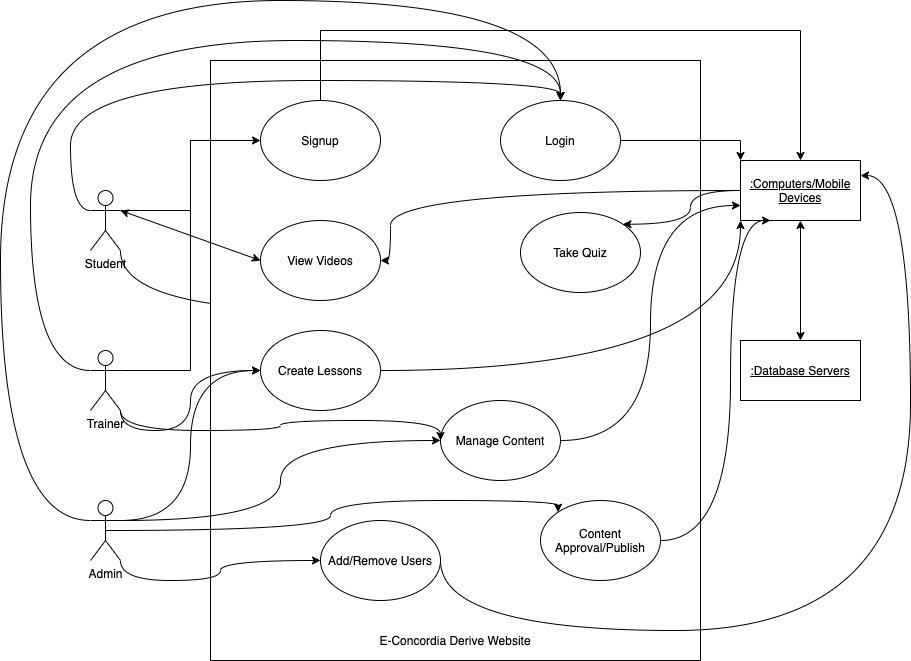
\includegraphics[scale=0.3]{UCM.png}
    \caption{UML Use Case Diagram}
    \label{fig:my_label}
\end{figure}

\subsection{UML Sequence Diagram}
\begin{figure}[htb!]
    \centering
    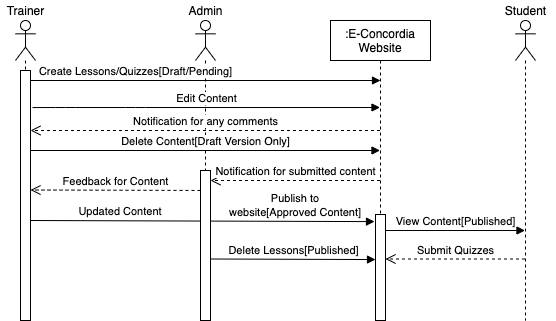
\includegraphics[scale=0.6]{SD.png}
    \caption{UML Sequential Diagram}
    \label{fig:my_label}
\end{figure}

\subsection{UML Activity Diagram}
\begin{figure}[htb!]
    \centering
    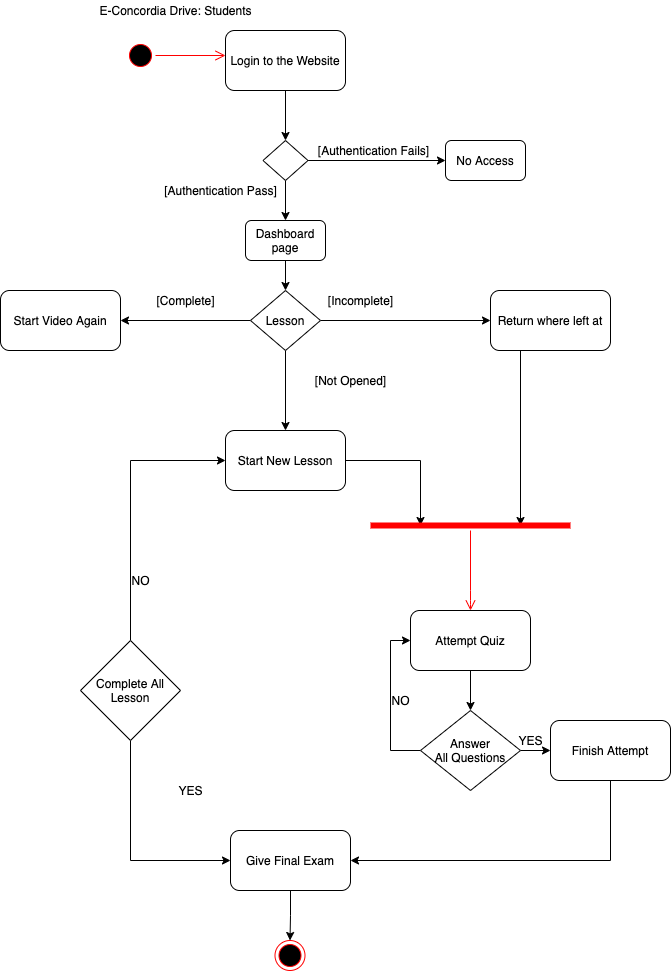
\includegraphics[scale=0.5]{AD.png}
    \caption{UML Activity Diagram}
    \label{fig:my_label}
\end{figure}

\section{Appendix}
\begin{table}[htb!]
    \centering
    \begin{tabular}{|p{5.5cm}|p{6.5cm}|}\hline
    \textbf{Section} & \textbf{Time Spent} \\ \hline
    Introduction & 0.5 hours \\ \hline
    Actors & 0.5 hours \\ \hline
    Use Case Model & 10 hours \\ \hline
    UML Diagrams & 1.5 hours \\ \hline
    \textbf{Total} & \textbf{12.5 hours} \\ \hline
\end{tabular}
    \caption{Appendix - Chapter 1}
    \label{tab:my_label}
\end{table}


\chapter{Supplementary Specification}
\section{ Introduction}
In this section we define the purpose, scope, all the definitions, acronyms and abbreviations and references.
\subsection{ Purpose}
The purpose of this document is define the requirements of E-Concordia Drive website, which is an e-learning platform where students prepare for their driving exams. This supplementary specification document lists the requirements that are not listed in the use case model document. The UCM and SS documents capture the whole requirements and form a final SRS.
\subsection{ Scope}
This SS documents applies to E-Concordia Drive website which will be developed by Chronos Tech Solutions. They will develop a client server system which will create the interface between mobile devices and EDC servers.\\[0.2cm]

E-Concordia drive is an E-learning platform for students to learn \& practice driving lessons to obtain a license. It has got three main Users: Trainer, Student and Administrator (quality). Admin edits, comments, approves and publishes  lessons uploaded by a trainer.  Once approved the content is ready to be viewed by students.\\[0.2cm]
This specification defines the non-functional requirements of the system; such as reliability, usability, performance, and supportability as well as functional requirements that are common across a number of use cases.
\subsection{ Definitions, Acronyms, Abbreviations}
Project Glossary is defined in \hyperref[sec:Glossary]{section 9}
%\nameref{sec:Glossary}
%\autoref{sec:Glossary}
\subsection{ References}
\begin{enumerate}
    \item {\footnotesize REST API Tutorial \textit{https://restfulapi.net/rest-architectural-constraints/}}
    \item {\footnotesize T.S Lehri, \textit{Vision Document E-Concordia Drive}, Summer 2021 SOEN 6481}
    \item {\footnotesize Dr. R.Morales, \textit{Trainer Wireframe}, SOEN 6481}
    \item {\footnotesize Dr. R.Morales, \textit{Student Wireframe}, SOEN 6481}
    \item {\footnotesize Dr. R.Morales, \textit{Admin Wireframe}, SOEN 6481}
    \item {\footnotesize Use Case Model - Student Registration \textit{UC001}, Summer 2021, E-Concordia Drive}
    \item {\footnotesize Use Case Model - Traner Registration \textit{UC002}, Summer 2021, E-Concordia Drive}
    \item {\footnotesize Use Case Model - Read Content of Dashboard \textit{UC003}, Summer 2021, E-Concordia Drive}
    \item {\footnotesize Use Case Model - View Videos by students \textit{UC004}, Summer 2021, E-Concordia Drive}
    \item {\footnotesize Use Case Model - Students take quiz \textit{UC005}, Summer 2021, E-Concordia Drive}
    \item {\footnotesize Use Case Model - Create Lesson \textit{UC006}, Summer 2021, E-Concordia Drive}
    \item {\footnotesize Use Case Model - Insert Content to Lesson \textit{UC007}, Summer 2021, E-Concordia Drive}
    \item {\footnotesize Use Case Model - Pending Lessons \textit{UC008}, Summer 2021, E-Concordia Drive}
    \item {\footnotesize Use Case Model - Draft Lessons \textit{UC009}, Summer 2021, E-Concordia Drive}
    \item {\footnotesize Use Case Model - Edit/Delete Lessons \textit{UC010}, Summer 2021, E-Concordia Drive}
    \item {\footnotesize Use Case Model - Notification for any Changes \textit{UC011}, Summer 2021, E-Concordia Drive}
    \item {\footnotesize Use Case Model - Admin Dashboard \textit{UC012}, Summer 2021, E-Concordia Drive}
    \item {\footnotesize Use Case Model - Manage Trainer \textit{UC013}, Summer 2021, E-Concordia Drive}
    \item {\footnotesize Use Case Model - Manage Students \textit{UC014}, Summer 2021, E-Concordia Drive}
    \item {\footnotesize Use Case Model - Manual Registrations \textit{UC015}, Summer 2021, E-Concordia Drive}
    
\end{enumerate}

\section{ Functionality}
This section lists the functional requirements that are common to more than one use case.
\subsection{Error Logs}
\begin{enumerate}
    \item A system error log should be maintained and shared with maintenance every night.
    \item All the errors will be logged in ERR\_LOGS table of the database 
    \item Error messages should have codes and description like ERROR123 - Taking more than usual buffer time.
    \item Error log file will be sent by system 2 hours before maintenance time and errors will be resolved during maintenance time.
\end{enumerate}

\subsection{Remote Access}
All the functionalities should be available to the users if they have a supporting device and internet connection.

\section{ Usability}
This section includes all the requirements that affect the usability of the website/app(for future).
\subsection{Training Time}
\begin{enumerate}
    \item All the new trainers should be provided 1 week training to familiarize them with the website.
    \item All the students will be given walk-through when they first visit the website.
\end{enumerate}

\subsection{Industry Standards}
Website will follow IBM CUA standards and IEC Reliability standards for touchscreen devices.

\subsection{Chat Bots}
There will be a chat bot on each page and users can chat with the CSR if they encounter an issue. 

\subsection{Multiple Systems/Web-Browser Support}
If a mobile app is made it should be working on below systems:
\begin{enumerate}
    \item iOS(iPhone, iPad)
    \item MacOSX (11.0 and up)
    \item Android
    \item Windows 8/10
\end{enumerate}

\section{ Reliability}
This section lists down all the reliability requirements for the system.
\subsection{Availability, MTBF, MTTR, MDR}
\begin{enumerate}
    \item \textbf{Availability:}
    \begin{itemize}
        \item System will be available 24/7 for all the users.
        \item System will have a downtime of 2 hours on every $2\textsuperscript{nd}$ Saturday of the month for maintenance.
        \item All the Error logs will be handled by maintenance team every day.
    \end{itemize}
    \item \textbf{Mean Time Between Failure:} MTBF shall exceed 500 hours.
    \item \textbf{Mean Time to Repair:} MTTR should be 30 minutes
    \item \textbf{Maximum bug or defect rate:} Maximum bug rate should be 5/KLOC. Categories of defects will be Critical, High Medium and Low(defined in glossary.
\end{enumerate}


\section{ Performance}
This section will list down all the performance requirements of the system.
\subsection{Response Time}
System should be able to complete 90\% transactions in 3 minutes
\subsection{Throughput}
System should be able to complete 100 transactions per second.
\subsection{Capacity}
System should be able to handle 350000 customers at any given time.
\subsection{Database/Server response time}
The system shall provide access to the EDC server with no more than a 10 second latency.
\subsection{Resource Utilization:} As it is a web application there will be very minimal resource utilization of a device. In future if an application is made it will require 200MB of disk space and enough storage space if downloadable resources are made available.

\section{ Supportability}
This section covers the supportability requirements of the system.
\begin{enumerate}
    \item System is supported on the readily web browsers in the market.
    \item If an application is made in future it will be downloadable on devices supporting OS listed in subsection 3.4 .
\end{enumerate}

\section{ Design Constraints}
This section lists the Design constraints of the system.
\subsection{Languages Supported:}
Videos uploaded will support English, Arabic, French, Hindi, Chinese, Italian for now. There will be a room for language support expansion.
\subsection{Development tools:}
Development tools used are \textbf{phpStrom} and \textbf{MySQL}.
\subsection{Management tools:}
\begin{enumerate}
    \item \textbf{Defect Management:} JIRA
    \item \textbf{CI/CD:} Github
    \item \textbf{Documentation:} Overleaf/Latex
\end{enumerate}
\subsection{Architectural Constraints:}
\begin{enumerate}
    \item Because this is a client server based application, the client and server application must be able to evolve separately without any dependency on each other.
    \item All the webpages should be cacheable to improve the performance on client end and better scalability on the server side.
\end{enumerate}


\section{ Online User Documentation and Help System Requirement}
\begin{enumerate}
    \item Screens should be interactive to make it easy to use on touch screen devices.
    \item Contact us information should be provided.
    \item A user should be guided through the system when they first login.
    \item A help document should be in place for the help later on.
\end{enumerate}

\section{ Glossary}
\label{sec:Glossary}
\subsection{Definitions}
\begin{longtable}{|p{4.5cm}|p{6.5cm}|}\hline
    \textbf{Name} & \textbf{Description}  \\ \hline
         User& End User of the system which includes student, trainer and admin\\ \hline
         Student& Person who registers to prepare for the driving test.\\ \hline
         Trainer& Person who is a driving instructor and creates content for students.\\ \hline
         Admin& Person who is also a QA and manages the driving school.\\ \hline
         Developer& Person responsible for the development of website\\ \hline
         Tester& Person reponsible for testing the code\\ \hline
         Data& \begin{itemize}
             \item \textbf{Definition 1} All the content on website.
             \item \textbf{Definition 2}Also details of users registered.
         \end{itemize}\\ \hline
         System& \begin{itemize}
             \item \textbf{Definition 1} E-Concordis Drive Website
             \item \textbf{Definition 2}A computer/mobile device
         \end{itemize}\\ \hline
         Server& The system which provides resources, data and services to other systems\\ \hline
         Quality Check & To verify if the content uploaded is correct\\ \hline
         Pending& Lesson is under review by the trainer and admin.\\ \hline
         Draft& Initial stages where person workig on content can edit it.\\ \hline
         Published& Content is made available for students.\\ \hline
         \caption{Definitions.\label{long}}\\
\end{longtable}

\subsection{Acronyms and Abbreviations}
\begin{longtable}{|p{4.5cm}|p{6.5cm}|}\hline
    \textbf{Acronym} & \textbf{Description}  \\ \hline
    MVC & Model View Controller \\ \hline
    MTTR & Mean Time to Repair \\ \hline
    MTBF & Mean Time to Failure \\ \hline
    KLOC & Tjousand Lines of Code \\ \hline
    IBM & International Business Machine \\ \hline
    IEC & International Electrotechnical Commission \\ \hline
    CUA & Common User Access\\ \hline
    SRS & Software Requirement Specifications\\ \hline
    SS & Supplementary Specifications\\ \hline
    LTR and RTL & Left-to-Right and Right-to-Left\\ \hline
    UCM& Use Case Model\\ \hline
    UML& Unified Modelling Language\\ \hline
         \caption{Acronyms and Abbreviation.\label{long}}\\
\end{longtable}

\section{Appendix}
\begin{table}[htb!]
    \centering
    \begin{tabular}{|p{5.5cm}|p{6.5cm}|}\hline
    \textbf{Section} & \textbf{Time Spent} \\ \hline
    Introduction & 1 hours \\ \hline
    Functionality & 1 hours \\ \hline
    Usability & 1 hours \\ \hline
    Reliability & 0.5 hours \\ \hline
    Performance & 1 hours \\ \hline
    Supportability & 0.5 hours \\ \hline
    Design Constraints & 1 hours \\ \hline
    ReliaOnline User Documentation and Help System Requirementbility & 0.5 hours \\ \hline
    Glossary & 1 hours \\ \hline
    \textbf{Total} & \textbf{7.5 hours} \\ \hline
\end{tabular}
    \caption{Appendix - Chapter 2}
    \label{tab:my_label}
\end{table}

\end{document}

